\documentclass[tikz,border=0pt]{standalone}

\usepackage[T1]{fontenc}
\usepackage{latexsym}
\usepackage{amsmath}
\usepackage{amsthm}
\usepackage{amssymb}
\usepackage{xspace}

\usepackage{graphicx}

\usepackage{tikz,pgf}
\usepackage{ctable} % for \specialrule command
\usetikzlibrary{shapes,arrows,automata,positioning,matrix,shapes,shadows,calc,decorations.markings,fit}

\providecommand{\jlcm}{\mbox{\textit{j}LCM}\xspace}
\providecommand{\toppi}{\mbox{\textsc{TopPI}}\xspace}
\providecommand{\capa}{\mbox{\textsc{CAPA}}\xspace}
\providecommand{\datalyse}{\mbox{\textsc{Datalyse}}\xspace}

\providecommand{\demoassoc}{\texttt{demo\-\_assoc}\xspace}
\providecommand{\prodassocreceipt}{\texttt{prod\-\_assoc\-\_receipt}\xspace}
\providecommand{\prodassocclient}{\texttt{prod\-\_assoc\-\_client}\xspace}

\tikzset{
    rulesTable/.style={
        matrix of nodes,
        row sep=-\pgflinewidth,
        column sep=-\pgflinewidth,
        nodes={
            rectangle,
            draw=black,
            align=center
        },
        minimum height=1em,
        minimum width=1em,
        text width=1em,
        text depth=0.5ex,
        text height=1ex,
        nodes in empty cells,
        %%
        every even row/.style={
            nodes={fill=black!30}
        },
        row 1/.style={
            nodes={
                fill=black!60,
                text=white,
                font=\small\bfseries
            }
        }
    }
}
\tikzset{element/.style={rectangle,
        inner sep=0pt,
        minimum width=1mm,
        draw=black,
        top color=blue!20!white!20,
        bottom color=blue!70!white,
}}

\tikzstyle{doc}=[%
	draw,
	thick,
	align=center,
	color=black,
	shape=rectangle,
	minimum width=10mm,
	minimum height=18.2mm,
	inner sep=2ex
]

\tikzset{
	comp/.style = {
		minimum width  = 3.5cm,
		minimum height = 2cm,
		text width     = 3.5cm,
		inner sep      = 0pt,
		text           = green,
		align          = center,
		font           = \Huge\bfseries,
		transform shape,
		thick
	},
	monitor/.style = {draw = none, xscale = 18/16, yscale = 11/9},
	display/.style = {shading = axis, left color = black!60, right color = black},
	ut/.style      = {fill = gray}
}

\tikzset{
	computer/.pic = {
		\node(-m) [comp, pic actions, monitor]
		{\phantom{\parbox{\linewidth}{\tikzpictext}}};
		\node[comp, pic actions, display,align=center] {\tikzpictext};
		\begin{scope}[x = (-m.east), y = (-m.north)]
			\path[pic actions, draw = none]
			([yshift=2\pgflinewidth]-0.1,-1) -- (-0.1,-1.3) -- (-1,-1.3) --
			(-1,-2.4) -- (1,-2.4) -- (1,-1.3) -- (0.1,-1.3) --
			([yshift=2\pgflinewidth]0.1,-1);
			\path[ut]
			(-1,-2.4) rectangle (1,-1.3)
			(-0.9,-1.4) -- (-0.7,-2.3) -- (0.7,-2.3) -- (0.9,-1.4) -- cycle;
			\path[pic actions, fill = none]
			(-1,1) -- (-1,-1) -- (-0.1,-1) -- (-0.1,-1.3) -- (-1,-1.3) --
			(-1,-2.4) coordinate(sw)coordinate[pos=0.5] (-b west) --
			(1,-2.4) -- (1,-1.3) coordinate[pos=0.5] (-b east) --
			(0.1,-1.3) -- (0.1,-1) -- (1,-1) -- (1,1) -- cycle;
			\node(-c) [fit = (sw)(-m.north east), inner sep = 0pt] {};
		\end{scope}
	}
}


\begin{document}


  % Define the layers to draw the diagram
  \pgfdeclarelayer{background}
  \pgfdeclarelayer{backgroundFore}
  \pgfdeclarelayer{foreground}
  \pgfsetlayers{background,backgroundFore,main,foreground}



  % Define block styles used later

  \tikzstyle{sensorNoShadow}=[draw, fill=blue!20, text width=6em,
      text centered, minimum height=2.5em]

  \tikzstyle{trans} = [cylinder, draw, minimum height=6em, minimum width=5em,
  fill=black!20, shape aspect=0.25, shape border rotate=90, text width=5em, text centered, font=\normalsize]

  \tikzstyle{data} = [cylinder, draw, minimum height=5em, minimum width=4em,
  shape aspect=0.25, shape border rotate=90, text width=6em, text centered, fill=white,font=\normalsize]

  \tikzstyle{table} = [cylinder, draw, minimum height=5em, minimum width=4em,
  shape aspect=0.25, shape border rotate=90, text width=4.5em, font=\normalsize, text centered, fill=gray!10]

  \tikzstyle{process} = [sensorNoShadow, text width=12em, minimum height=8em, fill=black!20, text=black, font=\large]

  \tikzstyle{webapp} = [draw, inner sep=0pt, minimum height=0em]

  \tikzstyle{number} = [circle, radius=0.5em, fill=gray!160, draw, font=\normalsize, text=white]

  \tikzstyle{switch} = [sensorNoShadow, text width=10em, minimum height=2em,
  font=\bfseries, fill=red!70, text=black]

  \tikzstyle{jlcm} = [sensorNoShadow, text width=6em, fill=black!70,
  minimum height=3em, text=white, minimum width=14em, font=\normalsize]
  \tikzstyle{jlcmServer} = [sensorNoShadow,  fill=black!40, minimum height=7em, minimum width=1em]
  \tikzstyle{jlcmCluster} = [sensorNoShadow, fill=black!40, minimum height=7em, minimum width=8.5em]

  %\draw[draw=black,solid, -triangle 90,fill=black] (0,0) -- (0,3);

  \tikzset{
      big black arrow/.style={
          decoration={markings,mark=at position #1*\pgfdecoratedpathlength with {\arrow[scale=3,black]{>}}},
  		postaction={decorate},
          shorten >=-0.5pt},
      big black arrowSmall dashed/.style={
  		decoration={markings, mark=at position #1*\pgfdecoratedpathlength with {\arrow[scale=2,black]{>}}},
  		postaction={decorate},
          shorten >=0.0pt, dashed},
      big black arrow dashed/.style={
  		decoration={markings, mark=at position #1*\pgfdecoratedpathlength with {\arrow[scale=3,black]{>}}},
  		postaction={decorate},
          shorten >=0.4pt, dashed},
      big black arrow dotted/.style={
  		decoration={markings,mark=at position #1*\pgfdecoratedpathlength with {\arrow[scale=3,black]{>}}},
  		postaction={decorate},
          shorten >=0.4pt,dotted},
      big black dotted/.style={
  		decoration={markings,mark=at position #1*\pgfdecoratedpathlength with},
  		postaction={decorate},
          shorten >=0.4pt,dotted},
      big black dashed/.style={
  		decoration={markings,mark=at position #1*\pgfdecoratedpathlength with},
  		postaction={decorate},
          shorten >=0.4pt,dashed}
  }


  \begin{tikzpicture}

  	\coordinate (yOffset) at (0,-3.5);

  	\coordinate (offsetLeft) at (-4.5,4.0);
  	\coordinate (offsetRight) at (3.2,3.5);

  	\coordinate (offsetCylinder) at (-5.2,5.7);
  	\coordinate (xOffsetCylinder) at (1.5,0);




      %%%
      %%% PREPARTION
      %%% id: process, case1, case2, case3
      %%%
      \node (prep) [process, minimum width=11em,minimum height=11em] {};
      \node (case1) [switch] at ($(prep.160)+(2.2,0.2)$) {\demoassoc};
      \node (case2) [switch] at ($(prep.180)+(2.2,0.2)$) {\prodassocreceipt};
      \node (case3) [switch] at ($(prep.200)+(2.2,0.2)$) {\prodassocclient};
  	\path (prep.south)+(0,0.3) node [font=\large] {Preparation};

  	%%%
      %%% CUSTOMERS, SALES, TAXONOMY
      %%% id: customers, sales
      %%%
      \node [table] (customers) at ($(prep.west)+(offsetCylinder)$) {$\mathit{customers}$};
  	\node [table] (sales) at ($(customers.east)+(xOffsetCylinder)$) {$\mathit{sales}$};
      \node [table,yshift=-4.0cm] (taxonomy) at ($(customers)!0.5!(sales)$) {$\mathit{taxonomy}$};

      %%%
      %%% BOUNDING-BOX: ACQUISITION-AND-STORAGE
      %%% id: redBox
      %%%
      \begin{pgfonlayer}{backgroundFore}

  		\path (customers.north west)+(-0.1,0.4) node (boxDataTopLeft) {};
  		\path (sales.east|-taxonomy.south)+(+0.3,-0.5) node (boxDataBottomRight) {};
  		\node [rectangle,fit=(boxDataTopLeft) (boxDataBottomRight),fill=black!15,rounded corners,
  		draw=black!50] (redBox) {};
  	\end{pgfonlayer}

      %%%
      %%% BOUNDING-BOX-LABEL: ACQUISITION-AND-STORAGE
      %%%
  	\path (redBox.south)+(0,0.3) node [font=\large] (boxLabelAcquAndStore) {{\bf Acquisition/Storage}};

      %%%
      %%% RECEIPTS
      %%%
  	\node [table] (tickets) at ($(sales.north)+(0,3.5)$) {$\mathit{store}$\\$\mathit{receipts}$};

      %%%
      %%% ARROW: BATCH TRANSFER
      %%%
      \draw[out=270,in=90,big black arrow=0.99] (tickets.south) to node[number,above]{1} node[above,xshift=-1.8cm]{Batch Transfer} (sales.north);


      ;above,xshift=-1.5cm

      %%%
      %%% ARROW: ENRICHMENT
      %%%
      \draw[out=280,in=250,big black arrow dashed=0.5] (customers.south) to node[below](enrichment) {{Enrichment}} (sales.south);
      \node [number] (dot2) at ($(enrichment.east)+(0.5,0)$) {2};

      %%%
      %%% ARROW: SALES,TAXONOMY to PREP
      %%%
      \coordinate (taxonomyPivot) at ($(taxonomy.east)+(1.5,0)$);
      \coordinate (centerPivot) at (taxonomyPivot|-prep);
      \coordinate (centerPivotLifted) at ($(centerPivot)+(0,0.2)$);
      \coordinate (centerPivotUnder) at ($(centerPivot)+(0,-0.2)$);

      \draw [big black arrow=0.6] (sales.east) -- (sales-|centerPivot) -- (taxonomyPivot) -- (taxonomy-|prep.west);
      \draw [big black arrow=0.9] (taxonomy.east) -- (taxonomy-|prep.west);



  	%%%%%%%%%%%%%%%%%%%%%%%%%%%%%%%%%%%%%%%%%%%%%%%%%%%%%%%%%%%%%%%%%%%%%%
  	%%%%%%%%%%%%%%%%%%%%%%%%%%%%%%%%%%%%%%%%%%%%%%%%%%%%%%%%%%%%%%%%%%%%%%
  	%%%%%%%%%%%%%%%%%%%%%%%%%%% FINISH: PART I %%%%%%%%%%%%%%%%%%%%%%%%%%%
  	%%%%%%%%%%%%%%%%%%%%%%%%%%%%%%%%%%%%%%%%%%%%%%%%%%%%%%%%%%%%%%%%%%%%%%
  	%%%%%%%%%%%%%%%%%%%%%%%%%%%%%%%%%%%%%%%%%%%%%%%%%%%%%%%%%%%%%%%%%%%%%%






  	%%%
      %%% TRANSACTIONS
      %%% id: transactions
      %%%
  	\node [trans] (transactions) at ($(prep)+(4.4,0)$) {$\cal D$};
      %\node [number] (dot4) at ($(transactions)+(1,1.5)$) {4};

  	%%%
      %%% ARROW: PREPARATION 2 TRANSACTIONS
      %%%
  	\draw [big black arrow=0.99] (prep.east) -- (transactions.west);

      %%%
      %%% BOUNDING-BOX: PREPARATION
      %%% id: curation
      %%%
  	\begin{pgfonlayer}{background}
  		\path (prep.north west)+(-0.1,0.1) node (boxLTopLeft) {};
          \path (prep.south -| transactions.east)+(0.1,-0.5) node (boxLBottomRight) {};
  		\node [rectangle,fit=(boxLTopLeft) (boxLBottomRight),fill=black!5,
          rounded corners,
  		draw=black!50] (curation) {};
  	\end{pgfonlayer}

      %%%
      %%% BOUNDING-BOX-LABEL: PREPARATION
      %%%
  	\path (curation.south) +(0,0.3) node [font=\large] (boxL) {{\bf Curation}};


  	%%%%%%%%%%%%%%%%%%%%%%%%%%%%%%%%%%%%%%%%%%%%%%%%%%%%%%%%%%%%%%%%%%%%%%
  	%%%%%%%%%%%%%%%%%%%%%%%%%%%%%%%%%%%%%%%%%%%%%%%%%%%%%%%%%%%%%%%%%%%%%%
  	%%%%%%%%%%%%%%%%%%%%%%%%%% FINISH: PART II %%%%%%%%%%%%%%%%%%%%%%%%%%%
  	%%%%%%%%%%%%%%%%%%%%%%%%%%%%%%%%%%%%%%%%%%%%%%%%%%%%%%%%%%%%%%%%%%%%%%
  	%%%%%%%%%%%%%%%%%%%%%%%%%%%%%%%%%%%%%%%%%%%%%%%%%%%%%%%%%%%%%%%%%%%%%%






      %%%
      %%% JLCM
      %%% id: jlcm
      %%%
  	\node [jlcm] (jlcm) at ($(transactions.south)+(-1,-6)$) { };
    \node [jlcmServer, anchor=north west] (jlcmServer) at (jlcm.south west) { };
    \node [jlcmCluster, anchor=north east] (jlcmCluster) at (jlcm.south east) { };
    \node [below, align=center ,text=white, font=\large] (jlcmText) at (jlcm.north) {\jlcm \\ \toppi};
      \node [number] (dot5) at ($(jlcmText)+(2.8,0.7)$) {4};

      %%%
      %%% ARROW: TRANSACTIONS to JLCM
      %%%
      \draw [big black arrow=0.6] (transactions) -- (transactions.south |- jlcm.north);

      \begin{pgfonlayer}{foreground}
      	\pic(server) [
      		draw,
      		fill = gray!30,
      		pic text = {Server},
      		scale=0.3
      	] at ($(jlcmText)+(-1.7,-1.6)$) {computer};

        \pic(cluster) [
          draw,
          fill = gray!30,
          pic text = {},
          scale=0.15
        ] at ($(jlcmText)+(2,-1)$) {computer};
        \pic(cluster) [
          draw,
          fill = gray!30,
          pic text = {},
          scale=0.15
        ] at ($(jlcmText)+(0,-1)$) {computer};
        \pic(cluster) [
          draw,
          fill = gray!30,
          pic text = {},
          scale=0.15
        ] at ($(jlcmText)+(1,-1)$) {computer};

        \pic(cluster) [
      		draw,
      		fill = gray!30,
      		pic text = {},
      		scale=0.15
      	] at ($(jlcmText)+(2,-2)$) {computer};
        \pic(clusterCenter) [
      		draw,
      		fill = gray!30,
      		pic text = {},
      		scale=0.15
      	] at ($(jlcmText)+(0,-2)$) {computer};
        \pic(cluster) [
      		draw,
      		fill = gray!30,
      		pic text = {},
      		scale=0.15
      	] at ($(jlcmText)+(1,-2)$) {computer};
      \end{pgfonlayer}

      \node [below, align=center, font=\large] (ClusterLabel) at ($(jlcmText)+(1,-2.5)$) {Cluster};

      %%%
      %%% RULES
      %%% id: rules
      %%%
      \matrix(rules) at ($(jlcmServer.west)+(-2.5,0)$) [rulesTable,text width=3.7em,minimum width=3.7em] {
          $I$ & $sup(I)$\\
          \ldots & \ldots \\
          \ldots & \ldots\\
      };

      \path (jlcm.south |- rules.north)+(0,-0.1) node[anchor=north] (rulesPivotTop) {};

      %%%
      %%% ARROW: JLCM to RULES
      %%%
      \draw [big black arrow=1] (jlcmServer.west) -- (rules.east);

      %%%
      %%% BOUNDING-BOX: MINING
      %%% id: greenBox
      %%%
  	\begin{pgfonlayer}{background}
  		\path (rules.west |- jlcm.north)+(-0.2,0) node[] (boxRTopLeft) {};
  		\path (jlcmCluster.south east)+(0.2,-0.6) node[] (boxRBottomRight) {};
  		\node [rectangle,fit=(boxRTopLeft) (boxRBottomRight),fill=black!5,rounded corners,
  		draw=black!50] (greenBox) {};
  	\end{pgfonlayer}

      %%%
      %%% BOUNDING-BOX-LABEL: MINING
      %%%
  	\path (greenBox.south) +(0,0.3) node [font=\large] (boxG) {{\bf Mining}};



  	%%%%%%%%%%%%%%%%%%%%%%%%%%%%%%%%%%%%%%%%%%%%%%%%%%%%%%%%%%%%%%%%%%%%%%
  	%%%%%%%%%%%%%%%%%%%%%%%%%%%%%%%%%%%%%%%%%%%%%%%%%%%%%%%%%%%%%%%%%%%%%%
  	%%%%%%%%%%%%%%%%%%%%%%%%%% FINISH: PART III %%%%%%%%%%%%%%%%%%%%%%%%%%
  	%%%%%%%%%%%%%%%%%%%%%%%%%%%%%%%%%%%%%%%%%%%%%%%%%%%%%%%%%%%%%%%%%%%%%%
  	%%%%%%%%%%%%%%%%%%%%%%%%%%%%%%%%%%%%%%%%%%%%%%%%%%%%%%%%%%%%%%%%%%%%%%


      %%%
      %%% DATABASE
      %%% id: database
      %%%
      %\matrix(database) at ($(rules)+(-1,2.5)$) [rulesTable,text width=3.6em,minimum width=3.6em] {
      %    $A\rightarrow B$ & $sup(A)$ & $sup(B)$ & $sup(A,B)$ & $m_1(A,B)$ & $m_2(A,B)$ & \ldots\\
      %    \ldots & \ldots & \ldots & \ldots & \ldots & \ldots & \ldots\\
      %    \ldots & \ldots & \ldots & \ldots & \ldots & \ldots & \ldots\\
      %};
      %\node [number] (dot6) at ($(database.east)+(-1,1.2)$) {6};

      \node[webapp] (webapp) at ($(rules)+(-5.5,0)$) {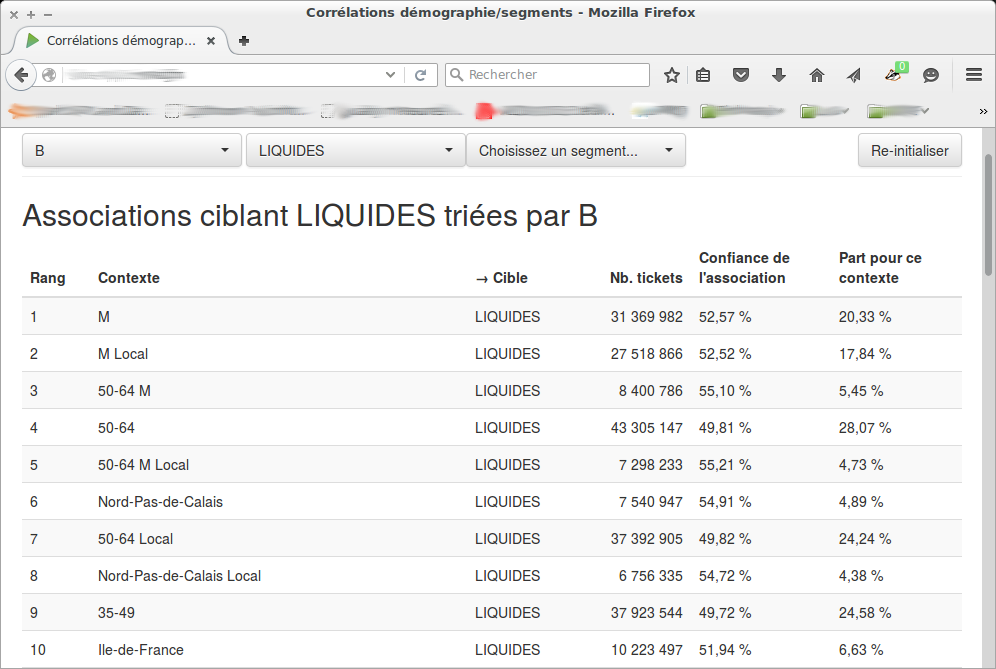
\includegraphics[scale=0.10]{../fig/screenshot_exploration.png}};
      \node [number] (dot6) at ($(webapp)+(1.7,1)$) {5};

      %%%
      %%% ARROW: DATABASE to WEBAPP
      %%%
      \draw [big black arrow=0.5] (rules) -- (webapp);

      %%%
      %%% BOUNDING-BOX: EXPLORATION
      %%% id: blueBox
      %%%
  	\begin{pgfonlayer}{background}
  	  \path (webapp.north west)+(-0.6,0.1) node (boxLTopLeft) {};
  	  \path (webapp.south east)+(0.6,-1) node (boxLBottomRight) {};
  	  \node [rectangle,fit=(boxLTopLeft) (boxLBottomRight),fill=black!5,
          rounded corners,
  	      draw=black!50] (blueBox) {};
  	\end{pgfonlayer}

      %%%
      %%% BOUNDING-BOX-LABEL: EXPLORATION
      %%%
      \path (webapp.south) +(0,-0.6) node [font=\large] (boxBL) {{\bf Exploitation} (\capa)};

      %%%
      %%% ARROW: RULES to DATABASE
      %%%
      %\coordinate (magicHinge) at ($(database.south-|rules)+(0,1)$);
      %\path (database.south -| magicHinge)+(0,-1) node[] (pointDatabase) {};
      %\path (rules.north -| magicHinge)+(0,-0.25) node[] (pointRules) {};
      %\path (database.south -| rules)+(0,0.2) node[] (pointDatabase) {};
      %\draw [big black arrow=0.8] ($(rules)+(0,-0.2)$) to node[above,xshift=0.2cm,yshift=0.1cm]{Enrichment with measures} (pointDatabase);
      %\draw[out=270,in=90,big black arrow=0.99] (tickets.south) to node[above,xshift=-0.6cm]{Batch Transfer} (sales.north);



      %%%%%%%%%%%%%%%%%%%%%%%%%%%%%%%%%%%%%%%%%%%%%%%%%%%%%%%%%%%%%%%%%%%%%%
  	%%%%%%%%%%%%%%%%%%%%%%%%%%%%%%%%%%%%%%%%%%%%%%%%%%%%%%%%%%%%%%%%%%%%%%
  	%%%%%%%%%%%%%%%%%%%%%%%%%% FINISH: PART IV %%%%%%%%%%%%%%%%%%%%%%%%%%%
  	%%%%%%%%%%%%%%%%%%%%%%%%%%%%%%%%%%%%%%%%%%%%%%%%%%%%%%%%%%%%%%%%%%%%%%
  	%%%%%%%%%%%%%%%%%%%%%%%%%%%%%%%%%%%%%%%%%%%%%%%%%%%%%%%%%%%%%%%%%%%%%%


      %%%
      %%% DECISION BOX
      %%% id: scenarioBox
      %%%
      \node [diamond, shape aspect=1.8, scale=0.8,draw,font=\large] (scenarioBox) at ($(prep.west)+(-4,-2)$)
      {\begin{tabular}{c}\setlength{\tabcolsep}{0pt} Scenario\\+\\Targets\end{tabular}};

      %%%
      %%% ANALYST
      %%% id: browser-c
      %%%
      \begin{pgfonlayer}{foreground}
      	\pic(browser) [
      		draw,
      		fill = gray!30,
      		pic text = {Analyst},
      		scale=0.4
      	] at ($(scenarioBox)+(0,-3)$) {computer};
      \end{pgfonlayer}
      %%%
      %%% ARROW: ANALYST to DECISION BOX
      %%%
      \coordinate (browserBoxRight) at ($(browser-c)$);
      %\coordinate (scenarioBoxLeft) at (scenarioBox|-browserBoxTop);
      \draw [big black arrow=1] (browserBoxRight) -- ($(scenarioBox.south)$);

      \coordinate (choicePivot) at ($(scenarioBox|-curation.south)+(0,-0.3)$);

      \coordinate (choicePivotTranslatedRight) at (choicePivot-|case1);
      \coordinate (choicePivotTranslatedLeft) at (choicePivot-|case3);

      \coordinate (lowprep) at ($(prep.west)+(0,-2)$);

      \draw [big black arrowSmall dashed=0.66] (scenarioBox.east) -- (lowprep);
      %\draw [big black arrowSmall dashed=0.90] (scenarioBox.north) -- (choicePivot) -- (choicePivotTranslatedRight) -- (case1);
      %\draw [big black arrowSmall dashed=0.66] (scenarioBox.north) -- (choicePivot) -- (choicePivotTranslatedLeft) -- (case3);
      %\draw [big black arrowSmall dashed=0.56] (choicePivotTranslated) -- (choicePivotTranslatedLifted) -- (case1);
      %\draw [big black arrowSmall dashed=0.56] (choicePivotTranslated) -- (choicePivotTranslatedSunk) -- (case3);
      %\draw [big black arrowSmall dashed=0.66] (choicePivotTranslated) -- (case2);


      \node [number] (dot3) at ($(scenarioBox)+(2.5,0)$) {3};

      %%%
      %%% ARROW: WEBAPP to ANALYST
      %%%
      %\coordinate (browser-c-shifted) at (browser.south);
      \draw [big black arrow=0.5] (browserBoxRight |- webapp.north) -- (browserBoxRight);

  	%%%%%%%%%%%%%%%%%%%%%%%%%%%%%%%%%%%%%%%%%%%%%%%%%%%%%%%%%%%%%%%%%%%%%%
  	%%%%%%%%%%%%%%%%%%%%%%%%%%%%%%%%%%%%%%%%%%%%%%%%%%%%%%%%%%%%%%%%%%%%%%
  	%%%%%%%%%%%%%%%%%%%%%%%% FINISH: DECISION BOX %%%%%%%%%%%%%%%%%%%%%%%%
  	%%%%%%%%%%%%%%%%%%%%%%%%%%%%%%%%%%%%%%%%%%%%%%%%%%%%%%%%%%%%%%%%%%%%%%
  	%%%%%%%%%%%%%%%%%%%%%%%%%%%%%%%%%%%%%%%%%%%%%%%%%%%%%%%%%%%%%%%%%%%%%%


  \end{tikzpicture}


\end{document}
